\documentclass[a4paper,10pt]{article}
\usepackage[utf8]{inputenc}
\usepackage{longtable}
\usepackage{tcolorbox}
\usepackage{tabularx}
\usepackage{amsmath}
\usepackage{capt-of}
\usepackage{supertabular}
\usepackage{url}
%opening
\title{Evaluating AIDA using hand annotated data}
\author{Aman Madaan}

\begin{document}

\maketitle

\begin{abstract}
Aim of this exercise was to benchmark AIDA by obtaining entity annotations on an already (hand) annotated dataset.
A low recall is observed, caused by failure to resolve ambiguitites correctly, and partially because of a large number
of extraneous hand annotated tags. For entities on which both the datasets agree, it is observed that for about 62\% entities, 
the number of annotations exactly match. For about 87\% of the entities, the number of annotations is within $\pm$ 5\% of the real value.


\end{abstract}

\section{Setup}
\subsection{Labeled data}
The ground truth data was taken from \url{http://www.cse.iitb.ac.in/soumen/doc/CSAW/Annot/}
\begin{itemize}
 \item 104 annotated files
 \item 3795 entities
 \item 19000 spots 
\end{itemize}

The annotations are available in XML format. A sample annotation is as follows : 
\begin{verbatim}
 <annotation>
	<docName>ganeshTestDoc.txt</docName>
	<userId>amitsingh</userId>
	<wikiName>Sachin Tendulkar</wikiName>
	<offset>420</offset>
	<length>9</length>
</annotation>
\end{verbatim}

\subsection{Getting annotations}
To compare how AIDA performs, we obtained annotations from AIDA in the same XML schema as
provided by CSAW team. The userId given was AIDA.
\begin{verbatim}
 <annotation>
<docName>ganeshTestDoc.txt</docName>
<userId>AIDA</userId>
<wikiName>Mike Denness</wikiName>
<offset>17</offset>
<length>12</length>
</annotation>
\end{verbatim}

Both the annotation files were then read into a hashmap of the form, $h(Entity) -> Count$. 
Maps for the two files were then scanned to generate the statistics presented in the next section.

\subsection{Annotated files}
XML file containing annotations for 104 files as above and for other 560 files is available at 
\url{www.cse.iitb.ac.in/~amanmadaan/store}

\subsection{Code}
The source code (without jar files) is hosted at \url{http://github.com/madaan/aida_benchmark}
\newpage
\section{Results}
Various statistics on the ratio of number of annotations made by AIDA to the number of annotations in the labeled data for a particular entity
are used as a metric of evaluation. 2 different setups were tried but results obtained were almost the same.
\subsection{Setup 1}
\subsubsectionmark{Details}
AIDA was run in \emph{FastLocalDisambiguation} mode. 
The Corpus used was yago trained from 2010 version of Wikipedia.
A total of $104$ documents were annotated.

\subsubsectionmark{Statistics}
\begin{center}
\bigskip \bigskip \bigskip \bigskip

\begin{tabular}{|l|l|}
 \hline
Total entities annotated by AIDA & 989\\ 
Total entities annotated by CSAW Team & 3795\\ 
Total entities common to both & 548\\ 
CSAW Entities missed by AIDA : (full list follows)  & 3247\\ 
AIDA Entities missed by CSAW : (full list follows)  & 441\\ 
\hline
\end{tabular}
\captionof{table}{Statistics on Entities}
\end{center}
\bigskip
\begin{center}
 \begin{figure}[h]
 \centering
 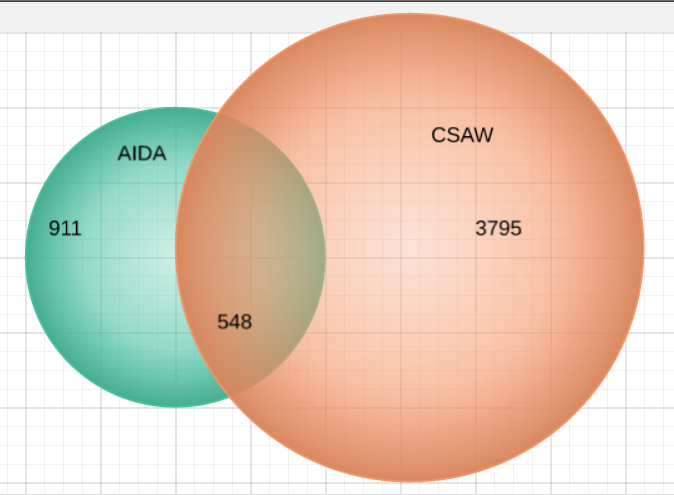
\includegraphics[bb=0 0 674 495,scale=0.3]{./venn.png}
 % venn.png: 674x495 pixel, 72dpi, 23.77x17.46 cm, bb=0 0 674 495
 \caption{Entities Annotated by CSAW and AIDA}
\end{figure}

 % venn.png: 674x495 pixel, 72dpi, 23.77x17.46 cm, bb=0 0 674 495
\end{center}

\bigskip 
\bigskip \bigskip 
\begin{center}
\bigskip
\begin{tabular}{|l|l|}
 \hline
$n$ & 548\\ 
$min$ & 0.03333333333333333\\ 
$max$ & 10.0\\ 
$mean$ & 1.1219961591723266\\ 
$std\_ dev$ & 0.9419811831930233\\ 
$median$ & 1.0\\ 
$skewness$ & 5.1513317988869085\\ 
$kurtosis$ & 34.719172895503725\\ 

\hline
\end{tabular}
\captionof{table}{Statistics for $score = \frac{\text{Annotations by AIDA}}{\text{Annotations by CSAW}}$}
\end{center}
\bigskip
\begin{figure}[h]
 \centering
 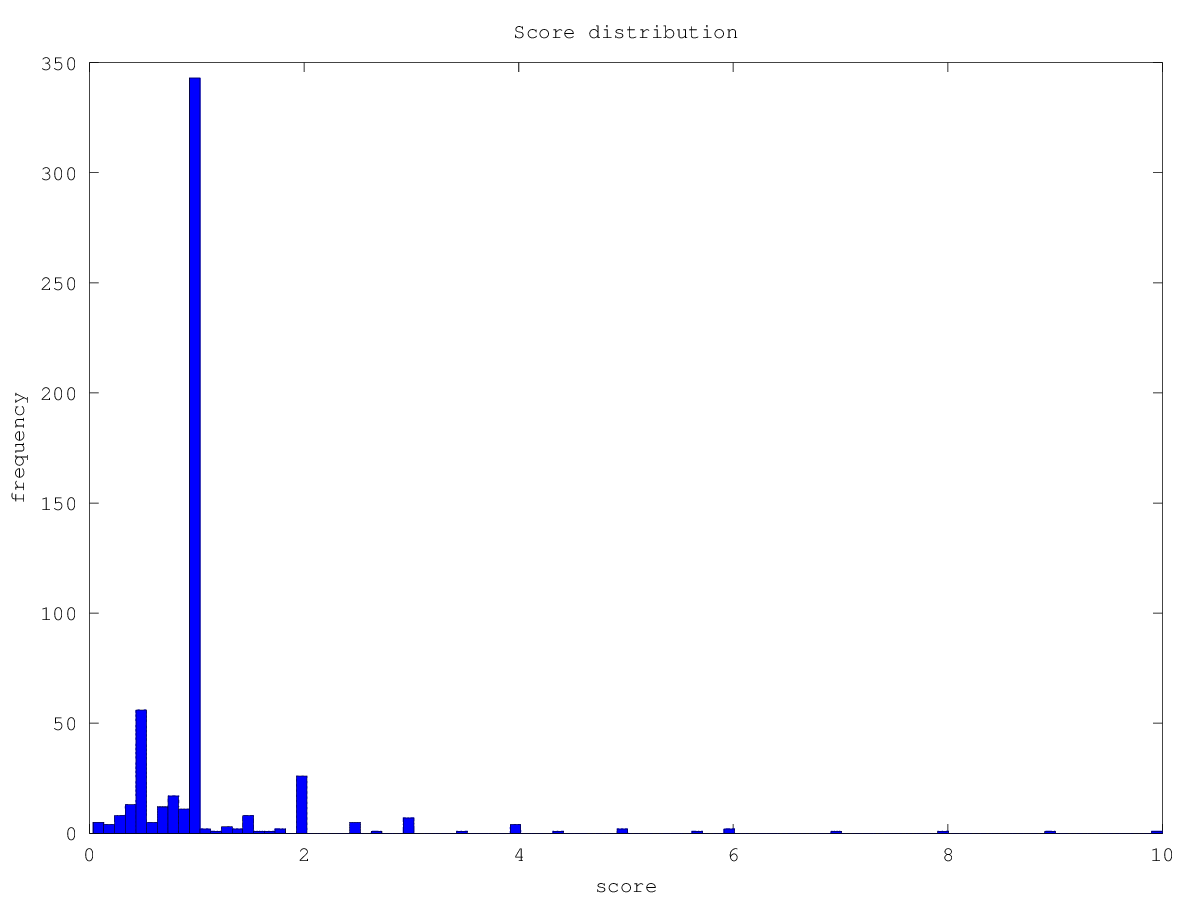
\includegraphics[bb=0 0 576 432,scale=0.5]{./dist.png}
 % dist.png: 1200x900 pixel, 150dpi, 20.32x15.24 cm, bb=0 0 576 432
 \caption{Distribution of scores for entities annotated by both CSAW and AIDA. CSAW and AIDA agree on 62\% entities}
\end{figure}
\bigskip
\begin{center}
\begin{tabular}{|l|l|}
 \hline
Score & Frequency\\
\hline
0.03 & 1 \\ 
0.17 & 1 \\ 
0.20 & 3 \\ 
0.25 & 7 \\ 
0.31 & 1 \\ 
0.33 & 7 \\ 
0.50 & 52 \\ 
0.60 & 1 \\ 
0.67 & 9 \\ 
1.00 & 342 \\ 
1.50 & 8 \\ 
2.00 & 26 \\ 
4.00 & 4 \\ 
4.33 & 1 \\ 
5.00 & 2 \\ 
5.67 & 1 \\ 
6.00 & 2 \\ 
7.00 & 1 \\ 
8.00 & 1 \\ 
9.00 & 1 \\ 
10.00 & 1 \\ \hline
\end{tabular}
\end{center}
\captionof{table}{Distribution of $score = \frac{\text{Annotations by AIDA}}{\text{Annotations by CSAW}}$}
\onecolumn
\bigskip 
\newpage
\newpage

\subsection{Setup 2}
\subsubsectionmark{Details}
AIDA was run in \emph{CocktailPartyDisambiguation} mode. 
The Corpus used was yago trained from \textbf{2012} version of Wikipedia.
A total of $104$ documents were annotated.

\subsubsectionmark{Statistics}
\begin{center}
\bigskip \bigskip \bigskip \bigskip

\begin{tabular}{|l|l|}
 \hline
Total entities annotated by AIDA & 911\\ 
Total entities annotated by CSAW Team & 3795\\ 
Total entities common to both & 510\\ 
CSAW Entities missed by AIDA : (full list follows)  & 3285\\ 
AIDA Entities missed by CSAW : (full list follows)  & 401\\ 
\hline
\end{tabular}
\captionof{table}{Statistics on Entities}
\end{center}

\bigskip 
\bigskip \bigskip 
\begin{center}

\begin{tabular}{|l|l|}
 \hline
$n$ & 510\\ 
$min$ & 0.045454545454545456\\ 
$max$ & 9.0\\ 
$mean$ & 1.1572691785583593\\ 
$std\_dev$ & 0.9019959891067724\\ 
$median$ & 1.0\\ 
$skewness$ & 4.558145927208736\\ 
$kurtosis$ & 27.172766135955523\\ 
\hline
\end{tabular}
\captionof{table}{Statistics for $score = \frac{\text{Annotations by AIDA}}{\text{Annotations by CSAW}}$}
\end{center}
\newpage

\section{Analysis}
 \bigskip
 \begin{itemize}
  \item \textbf{AIDA annotates 989 entities, but only 548 of them were also in CSAW}
  There can be several reasons for this :
  \begin{itemize}
  \item  \textbf{Ambiguity of tagging}. Gandhi was wrongly linked to ``Indira Gandhi'' and not ``Mahatma Gandhi'' at several places. \medskip
  
  \item \textbf{Different Wikipedia titles for same entity}. ``Reuters'' can be ``Thomson Reuters'' or ``the news agency''. 
  Since the comparison was based on the title of the Wikipedia page that is linked, such annotations fail to match. \medskip
  \item  \textbf{New Wikipedia pages} might have emerged since CSAW was annotated. For eg, Harald zur Hansen is present in the corpus
  but not tagged by CSAW team. \medskip
  \end{itemize}
  
  \item out of 548 matches, 342 \textbf{($62\%$)} were \emph{exactly} annotated. This means that AIDA performs as good as a human being for these cases.
   \medskip
  
 \item Annotated data had some discrepancies. In file 13OctAmitSport14.txt, only 1 out of 9 instances of 
 Steve Hodge was tagged. (Steve Hodge was mentioned by just the last name in 8 places)
 \medskip
 \item There were some extraneous tags. Words like Loss, Excellency, Utility, Year etc. were tagged with links
 to wiki pages. It is not exactly clear why such tags will be required. \textbf{The low recall}, ($0.2606, \frac{989}{3795}$)
seems to be caused by such extraneous tags.
  \medskip
 \item There was not much difference in AIDA's performance with both local and global disambiguation settings.
  \medskip
 \item Resolving ambiguities is still a big challenge. 
 \medskip
 \end{itemize}
\end{document}
% 